\chapter{Concluding Remarks}
\label{chap:conclusion}

%\epigraph{
%\textit{When information is cheap, attention becomes expensive.}
%}
%{
%--James Gleick, \textit{The Information}
%}
%
%\epigraph{
%\textit{Our task as men is to find the few principles that will calm the infinite anguish
%of free souls. We must mend what has been torn apart, make justice imaginable again in a
%world so obviously unjust, give happiness a meaning once more to peoples poisoned by the
%misery of the century. Naturally, it is a superhuman task. But superhuman is the term
%for tasks men take a long time to accomplish, that's all.}
%}
%{
%--Albert Camus, \textit{The Almond Trees}
%}

\epigraph{
    \textit{The point is there ain't no point.}
}
{
    --Cormac McCarthy, \textit{No Country for Old Men}
}

%\epigraph{
%    \textit{The more the universe seems comprehensible, the more it also seems pointless.
%    But if there is no solace in the fruits of our research, there is at least some consolation
%    in the research itself. Men and women are not content to comfort themselves with tales of
%    gods and giants, or to confine their thoughts to the daily affairs of life; they also build telescopes
%    and satellites and accelerators, and sit at their desks for endless hours working out the meaning of the
%    data they gather. The effort to understand the universe is one of the very few things that lifts
%    human life a little above the level of farce, and gives it some of the grace of tragedy.}
%}
%{
%    --Steven Weinberg, \textit{The First Three Minutes}
%}

\epigraph{
    \textit{The effort to understand the universe is one of the very few things that lifts
    human life a little above the level of farce, and gives it some of the grace of tragedy.}
}
{
    --Steven Weinberg, \textit{The First Three Minutes}
}

%%%%%%%%%%%%%%%%%%%%%%%%%%%%%%%%%%%%%%%%%%%%%%%%%%%%%%%%%%%%%%%%%%%%%%%%%%%%%%%%%%%%%%%%%%%%%%
%%%%%%%%%%%%%%%%%%%%%%%%%%%%%%%%%%%%%%%%%%%%%%%%%%%%%%%%%%%%%%%%%%%%%%%%%%%%%%%%%%%%%%%%%%%%%%
%%%%%%%%%%%%%%%%%%%%%%%%%%%%%%%%%%%%%%%%%%%%%%%%%%%%%%%%%%%%%%%%%%%%%%%%%%%%%%%%%%%%%%%%%%%%%%

\cite{FengNaturalness}

This dissertation has presented work related to the on-going upgrade of the forward muon system
of the ATLAS detector --- the New Small Wheel --- as well as two searches for BSM physics in dilepton final states.

\begin{figure}[!htb]
    \begin{center}
        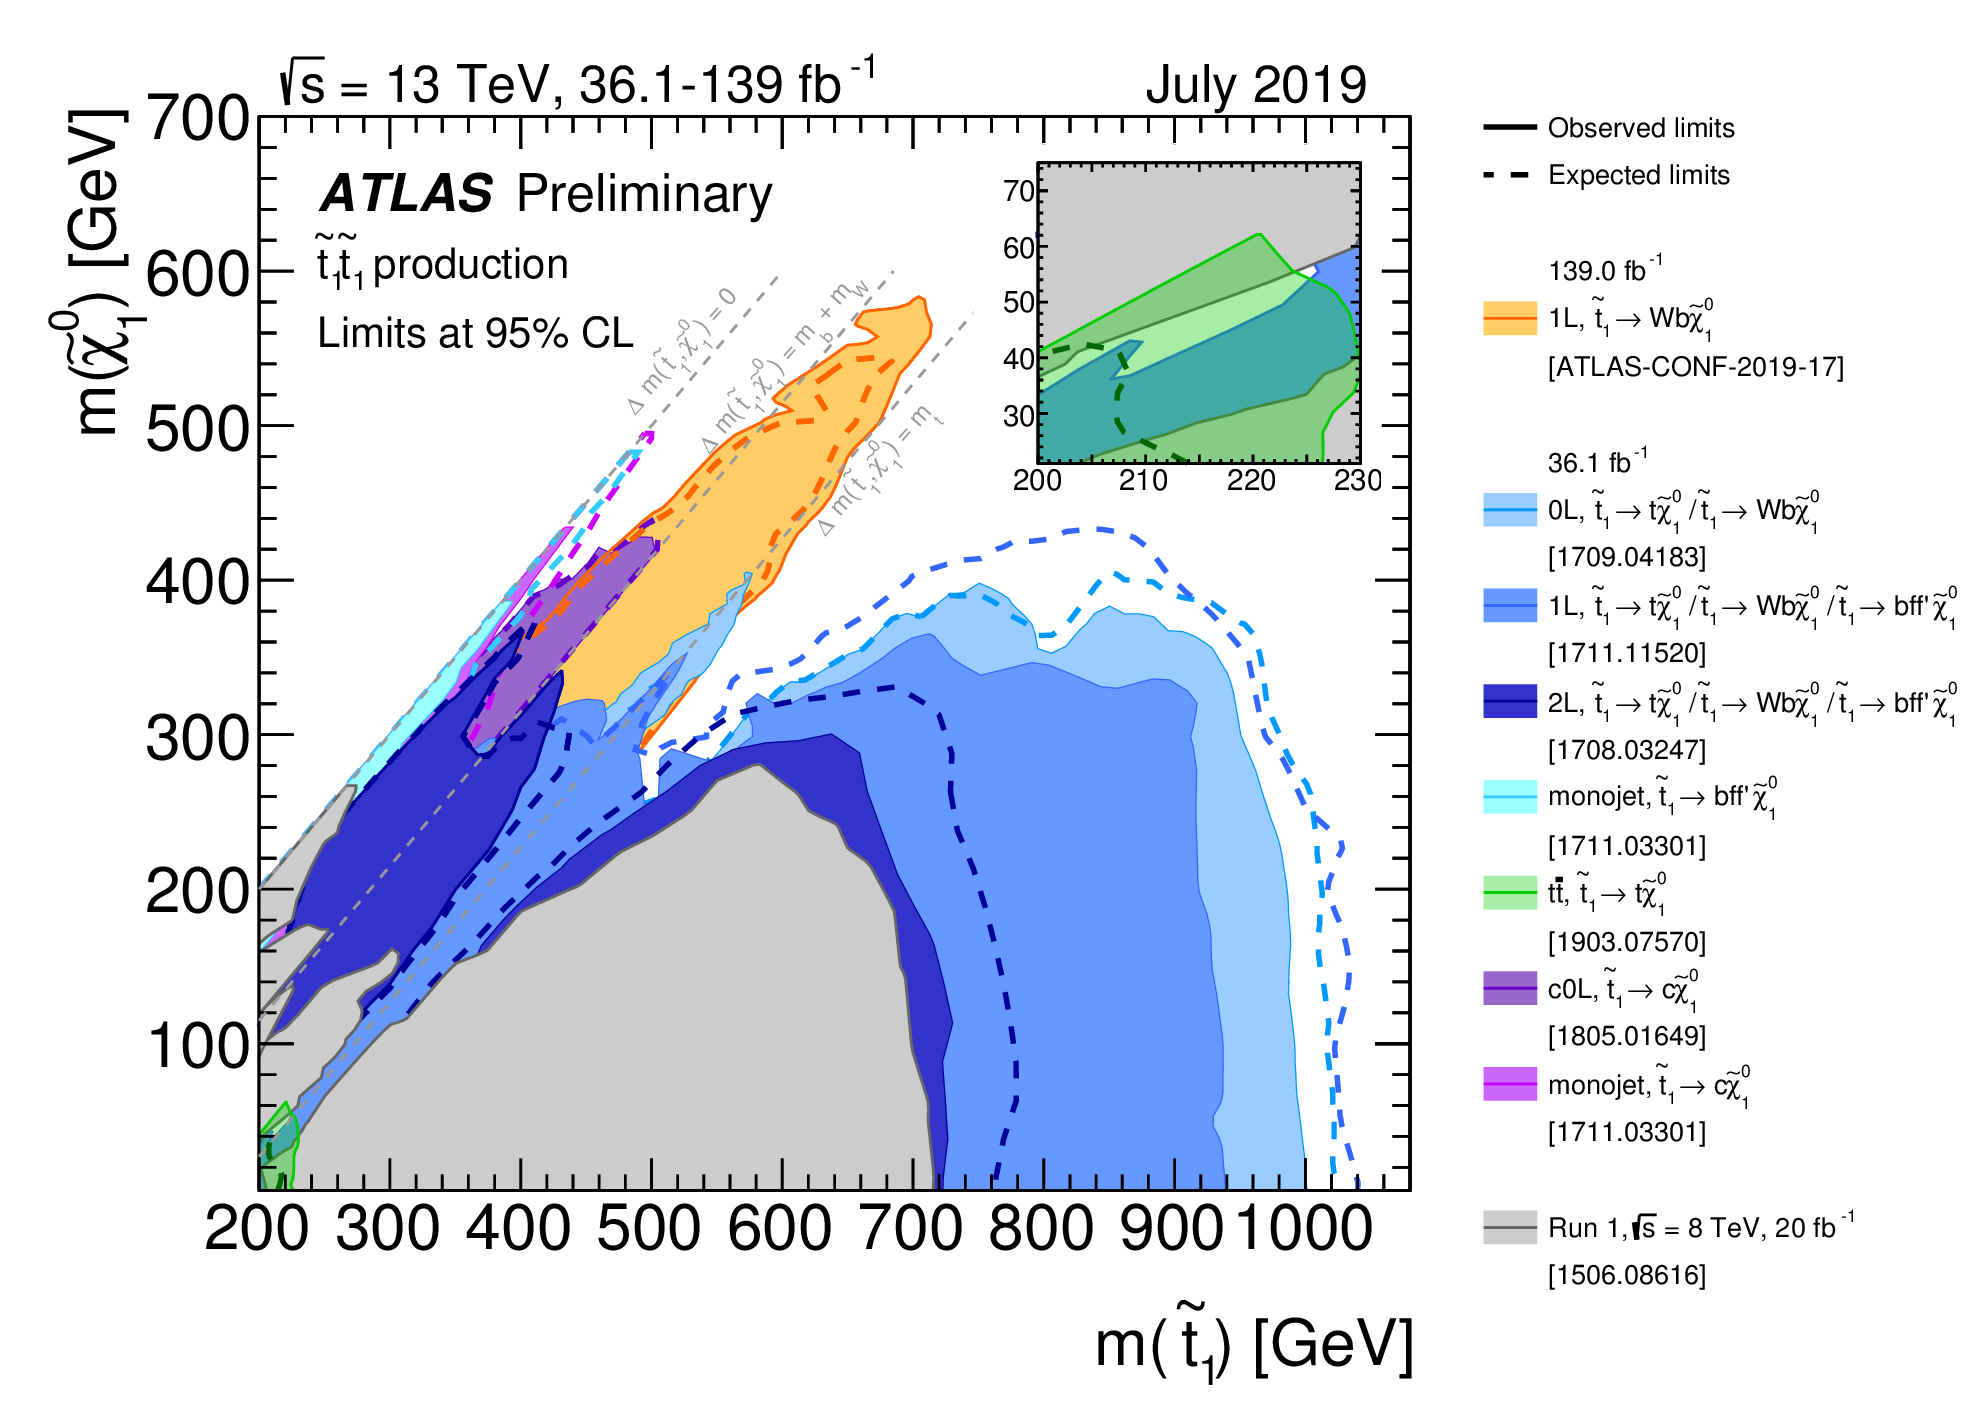
\includegraphics[width=0.85\textwidth]{figures/conclusion/ATLAS_SUSY_Stop_tLSP}
        \caption{
        }
        \label{fig:run2_stop_summary}
    \end{center}
\end{figure}
